\documentclass[compress]{beamer}
\usepackage[utf8]{inputenc}
\usepackage[T1]{fontenc}
\usetheme{Singapore}
\usecolortheme{default}
\usepackage{graphicx}

\begin{document}
\title{Verschlüsselung mit GPG}  
\author{Sokü \& friends}
\date{} 

\frame{\titlepage} 

\frame{
  \frametitle{Struktur}
  \tableofcontents
} 

\section{Motivation}
\label{sec:motivation}

\begin{frame}
  \frametitle{Warum das alles eigentlich?}

  \begin{itemize}[<+(1)->]
  \item Emails sind unsicher
  \item Nur wer ein bisschen die Technik versteht, kann sich bewusst
    verhalten
  \end{itemize}
\end{frame}

\section{Theorie}
\label{sec:theorie}
\begin{frame}
    \frametitle{\insertsection}
    \begin{description}
        \item[Verschlüsselung] Ich will nicht, dass alle wissen, was ich schreibe.
        \item[Authentifikation] Ich will mit der richtigen Person sprechen.
    \end{description}
\end{frame}

\subsection{Symmetrische und Asymmetrische Verschlüsselung}
\begin{frame}
  \frametitle{\insertsubsection}
  \begin{overprint}
    \onslide<1-4>
    \begin{description}
    \item[Symmetrische Verschlüsselung:] \alert{Ein} Schlüssel
      zum Verschlüsseln und wieder Entschlüsseln.
      
      \only<4>{Der Schlüssel muss
      sicher von der Senderin zum Empfänger gebracht werden. (alte
      Agentenfilme: Aktenkoffer mit Selbstzerstörung, das ist doch
      aufwändig)}
    \end{description}
    \onslide<5-7>
    \begin{description}
    \item[Asymmetrische Verschlüsselung:] Zwei
      Schlüssel: Ein \alert{öffentlicher} nur zum Verschlüsseln (darf
      auch den Bösen bekannt sein) und ein \alert{privater} zum
      Entschlüsseln (geheim, muss aber nicht mehr quer durch die Stadt
      getragen werden)
    \end{description}
    \onslide<8>
    \begin{description}
    \item[Wie geht das?] Mathe!  Zahlen multiplizieren geht leicht,
      Zahlen wieder aufteilen nicht.
    \end{description}
  \end{overprint}
  \vspace{1em}
  \begin{overlayarea}{\columnwidth}{8em}
    \includegraphics<2>[width=\columnwidth]{bilder/symmetric_schluessel.png}
    \includegraphics<3>[width=\columnwidth]{bilder/symmetric_text.png}
    \only<4>{
      \begin{center}
        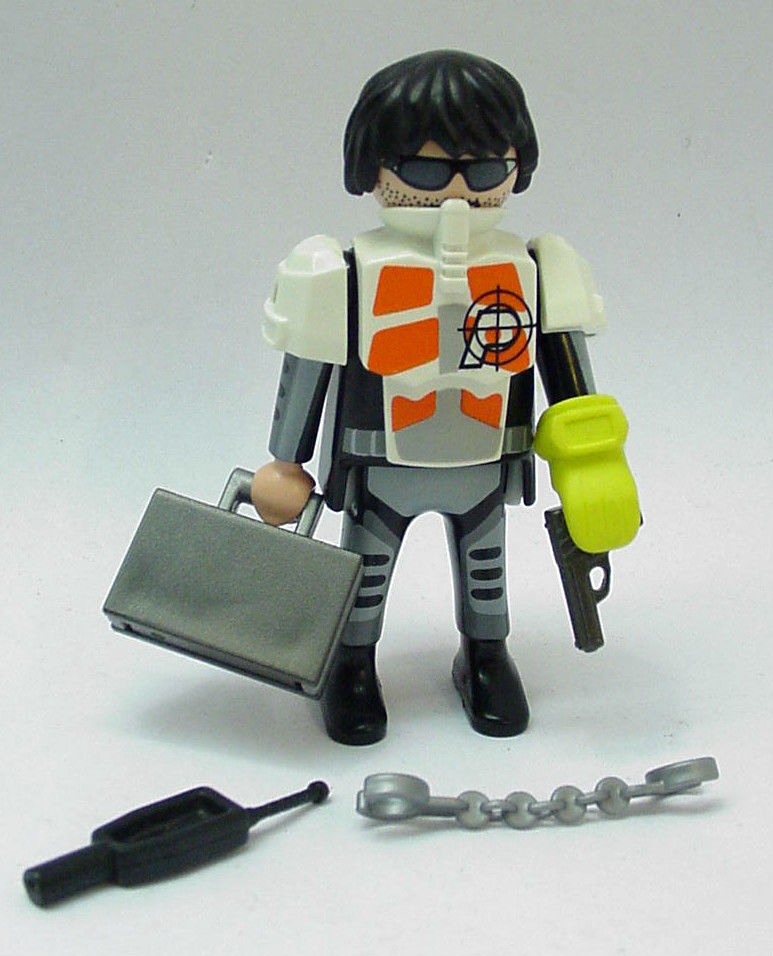
\includegraphics[height=9em]{bilder/agent_koffer.jpg}
      \end{center}
    }
    \includegraphics<6>[width=\columnwidth]{bilder/public_key_verfahren_schluessel.png}
    \includegraphics<7>[width=\columnwidth]{bilder/public_key_verfahren_text.png}
  \end{overlayarea}

\end{frame}

\subsection{Primzahlen rechnen}
\begin{frame}
  \frametitle{\insertsubsection}
  \begin{description}
  \item[Taschenrechner dabei?]
    \begin{itemize}
    \item 7 x 11 = ?
    \item 65 = ? x ? (5 x 13)
    \item 11251 x 2953 = 33224203
    \item 12883649 = ? (2957 x 4357) kann wohl niemand in unter einem
      Tag ausrechnen, auch mit Taschenrechner
    \end{itemize}
  \item[Verschlüsselung?] Das Produkt aus den zwei Primzahlen ist in
    etwa der öffentliche Schlüssel (auch die Geheimdienste können die
    Zahl nicht wieder aufspalten), die zwei kleinen Zahlen sind der
    private Schlüssel und müssen geheim bleiben.
  \end{description}
\end{frame}

\section{Theoretische Praxis}
\label{sec-1-1-4}

Schlüsselerstellung (Zufall), Schlüsselaustausch, Schlüsselserver,
Fingerprints, Signaturen (Keysigning-Parties), Widerrufszertifikat,
Email (Betreff, Header, Anhänge)

Abgrenzen zu:
\begin{itemize}
\item Festplattenverschlüsselung
\item Apps auf Handys/Smartphones, Chat
\item Anonymität
\end{itemize}
\section{Die Praxis in der Theorie}
\label{sec-1-1-5}

\begin{frame}
  \frametitle{\insertsection}
  Programme zum Verschlüsseln:

  \begin{description}
  \item[gpg] \alert{G}nu\alert{P}rivacy\alert{G}uard, ein Programm,
    das verschlüsseln kann.  Heißt auf Windows \alert{GPG4Win}.
  \item[Enigmail] Ein Plugin für das Thunderbird-Mailprogramm, das gpg
    verwendet, um Mails zu verschlüsseln.
  \end{description}

\end{frame}

GPG4Win, Enigmail, sonstige Programme

Screenshots: Installation, Schlüsselgenerierung
(Widerrufszertifikat!), Einrichtung Enigmail, Schlüssel hochladen,
Schlüssel runterladen, Mail versenden, Mail empfangen
\section{Praktische Praxis}
\label{sec-1-1-6}

\begin{itemize}
\item Runterladen/Verteilen
\item Installieren
\item \ldots{} (wie oben)
\end{itemize}

Vielleicht zuerst eine Mail an sich selber schreiben?
\section{Weiterführendes}
\label{sec-1-1-7}

\begin{itemize}
\item Skript?
\item Feedbackrunde
\item Weitere Wünsche?
\end{itemize}

\end{document}
